\subsection{Garanzia della qualità}
\subsubsection{Scopo}
Stabilire una metrica di valutazione precisa ed oggettiva per misurare il prodotto software garantendo un'informe livello di qualità per tutto il ciclo di vita del software.
\subsubsection{Aspettative}
L'aspettativa del processo di garanzia della qualità è che quest'ultimo aiuti il \Gruppo{} ad essere \glo{sistematico}, \glo{disciplinato} e \glo{quantificabile}, ai fini di:
\begin{itemize}
    \item Garantire la qualità nel prodotto software da realizzare;
    \item Soddisfare le richieste del proponente e del committente;
    \item Migliorare le proprie capacità di gestione di un progetto software.
\end{itemize}
\subsubsection{Descrizione}
Il processo di garanzia della qualità è un processo fornisce un'adeguata garanzia che i prodotti e i processi software nel ciclo di vita del progetto siano conformi ai requisiti specificati e aderiscano ai piani stabiliti. La garanzia della qualità può essere interna o esterna a seconda che la prova della qualità del prodotto o del processo sia dimostrata all'interno del gruppo o all'utente finale.
\subsubsection{Attività}
\paragraph{Implementazione del processo}
\subsection{ISO/IEC 12207}
ISO/IEC 12207 è uno standard utilizzato per misurare la qualità dei \glo{processi}. Questa normativa è suddivisa in 3 parti
ed ognuna contiene dei sotto \glo{processi} e delle attività. Il tutto è riportato in seguito. 

\begin{figure}[h]
    \centering
    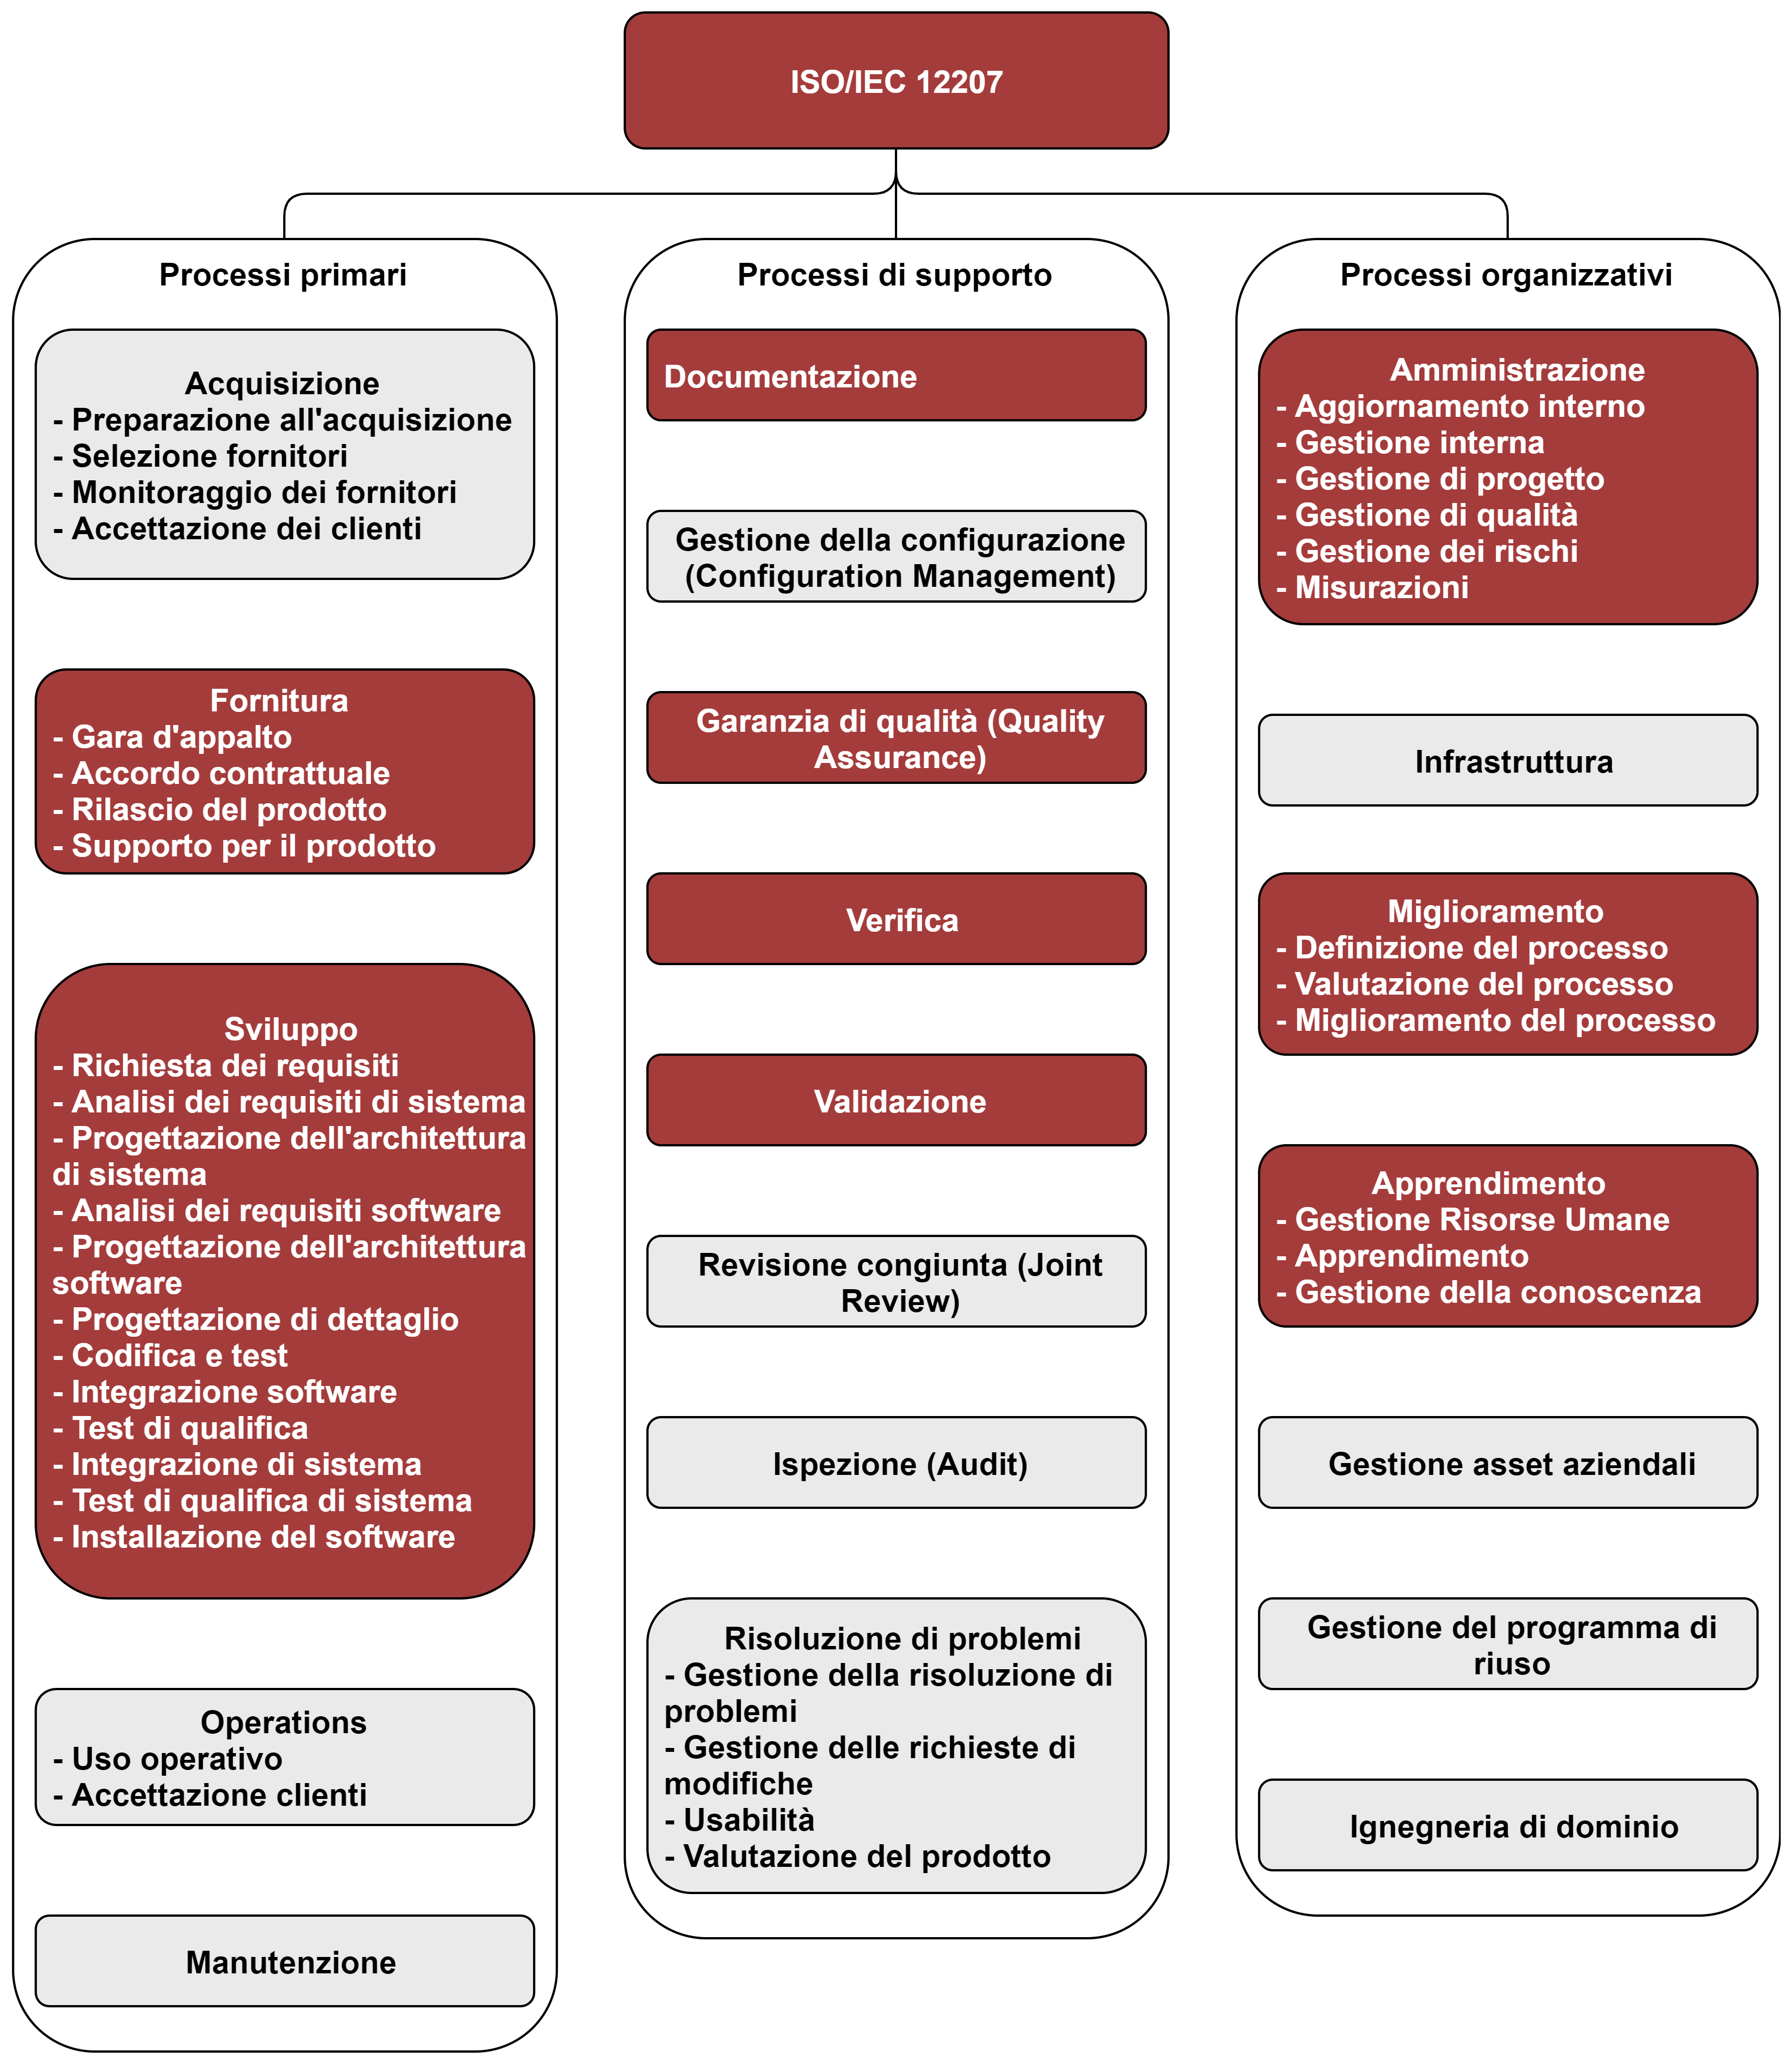
\includegraphics[scale=0.53]{Sezioni/Immagini/IsoIec12207.png}
    \caption{Schema dello standard ISO/IEC 12207. In rosso sono indicati i processi e le relative attività di interesse per il progetto.}
\end{figure}

\subsubsection{Processi primari}
Sono i \glo{processi} e le attività che fanno parte dello sviluppo del software e hanno lo scopo di soddisfare tutti i requisiti concordati con il cliente.

\paragraph{Sviluppo}\mbox{}\\ \\
Il \glo{processo} ha lo scopo di sviluppare un prodotto software, o un sistema basato sul software, che indirizzi le esigenze del cliente. \\
I risultati delle valutazioni dei \glo{processi} devono essere documentati.
\begin{itemize}
    \item \textbf{Analisi dei requisiti:} \\
    Lo sviluppatore deve valutare i requisiti software in base ai criteri elencati di seguito:
        \begin{itemize}
            \item Tracciabilità dei requisiti di sistema e progettazione del sistema;
            \item Coerenza esterna con i requisiti di sistema;
            \item Coerenza interna;
            \item \glo{Testabilità};
            \item Fattibilità della progettazione del software;
            \item Fattibilità di funzionamento e manutenzione.
        \end{itemize}
    \item \textbf{Pianificazione di dettaglio:} \\
    Lo sviluppatore deve sviluppare un progetto dettagliato per ciascun componente software. I componenti del software 
    devono essere perfezionati in livelli inferiori contenenti unità software che possono essere codificati, compilati 
    e testati. È necessario garantire che tutti i requisiti software siano assegnati dai componenti software 
    alle unità software.
    
    \item \textbf{Codifica:} \\
    Lo sviluppatore deve valutare il codice del software e i risultati dei test considerando i criteri elencati sotto:
    \begin{itemize}
        \item Tracciabilità ai requisiti e alla progettazione dell'articolo software;
        \item Coerenza esterna con i requisiti e il design dell'articolo software;
        \item Coerenza interna tra i requisiti dell'unità;
        \item Testare la copertura delle unità;
        \item Adeguatezza dei metodi e delle norme di codifica utilizzati;
        \item Fattibilità dell'integrazione e dei test del software;
        \item Fattibilità di funzionamento e manutenzione.   
    \end{itemize}
\end{itemize}

\subsubsection{Processi di supporto}
Sono i \glo{processi} e le attività che aiutano gli altri \glo{processi} nel raggiungimento del successo e nella qualità del progetto.

\paragraph{Documentazione}\mbox{}\\ \\
Il \glo{processo} di "Gestione della documentazione" garantisce lo sviluppo e la manutenzione delle informazioni prodotte e registrate relativamente al prodotto software. \\ \\
\textbf{Implementazione:} \\ 
Identifica i documenti da produrre durante il ciclo di vita del prodotto software;
deve essere sviluppato, documentato e implementato. La documentazione dovrà prevedere i seguenti punti: 
\begin{itemize}
    \item Titolo o nome;
    \item Scopo;
    \item Pubblico previsto;
    \item Procedure e responsabilità per input, sviluppo, revisione, modifica, approvazione, produzione, stoccaggio, distribuzione, manutenzione e gestione della configurazione;
    \item Programma per le versioni intermedie e finali.
\end{itemize}

\paragraph{Garanzia di qualità}\mbox{}\\ \\
Il \glo{processo} di "Assicurazione qualità" ha lo scopo di assicurare che tutti i prodotti di fase (work product) siano conformi con i piani e gli standard definiti.
\paragraph{Verifica}\mbox{}\\ \\
Il \glo{processo} di verifica ha lo scopo di confermare che ciascun work product o servizio realizzato da un \glo{processo} soddisfi i requisiti specificati. 
Il \glo{processo} di verifica deve essere integrato nei \glo{processi} di Sviluppo, Fornitura e Manutenzione. Se la verifica viene eseguita da terzi, questa viene definita come "\glo{Processo} di verifica indipendente".
\\
Il \glo{processo} deve essere verificato considerando i criteri elencati di seguito:
\begin{itemize}
    \item I requisiti di pianificazione del progetto sono adeguati e tempestivi;
    \item I \glo{processi} selezionati per il progetto sono adeguati, implementati, eseguiti come previsto, e conformi al contratto;
    \item Gli standard, le procedure e gli ambienti per i \glo{processi} del progetto sono adeguati;
    \item Il progetto è composto da personale qualificato capace di soddisfare le richieste del contratto.
\end{itemize}

\subsubsection{Processi organizzativi}
Sono i \glo{processi} e le attività che coprono gli aspetti organizzativi e di gestione delle risorse.

\paragraph{Gestione}\mbox{}\\ \\
Il \glo{processo} di gestione garantisce lo sviluppo e la manutenzione delle informazioni prodotte e registrate relativamente 
al prodotto software. L'amministratore prepara i piani per l'esecuzione del \glo{processo}.
I piani associati all'esecuzione del \glo{processo} devono contenere descrizioni: delle attività, dei compiti associati e
identificazioni dei prodotti software che verranno forniti. Questi piani devono rispettare i seguenti punti:
\begin{itemize}
    \item Programmi per il completamento tempestivo dei compiti;
    \item Risorse adeguate necessarie per eseguire i compiti;
    \item Assegnazione di compiti;
    \item Assegnazione di responsabilità;
    \item Quantificazione dei rischi associati ai compiti o al \glo{processo} stesso;
    \item Misure di controllo della qualità da applicare durante l'intero \glo{processo};
    \item Costi associati all'esecuzione del \glo{processo};
    \item Fornitura di ambiente e infrastruttura.
\end{itemize}

\subsection{ISO/IEC 9126}
Lo standard ISO/IEC 9126 si occupa di presentare le caratteristiche di qualità di un prodotto software e gli attributi che le compongono.

\begin{figure}[h]
    \centering
    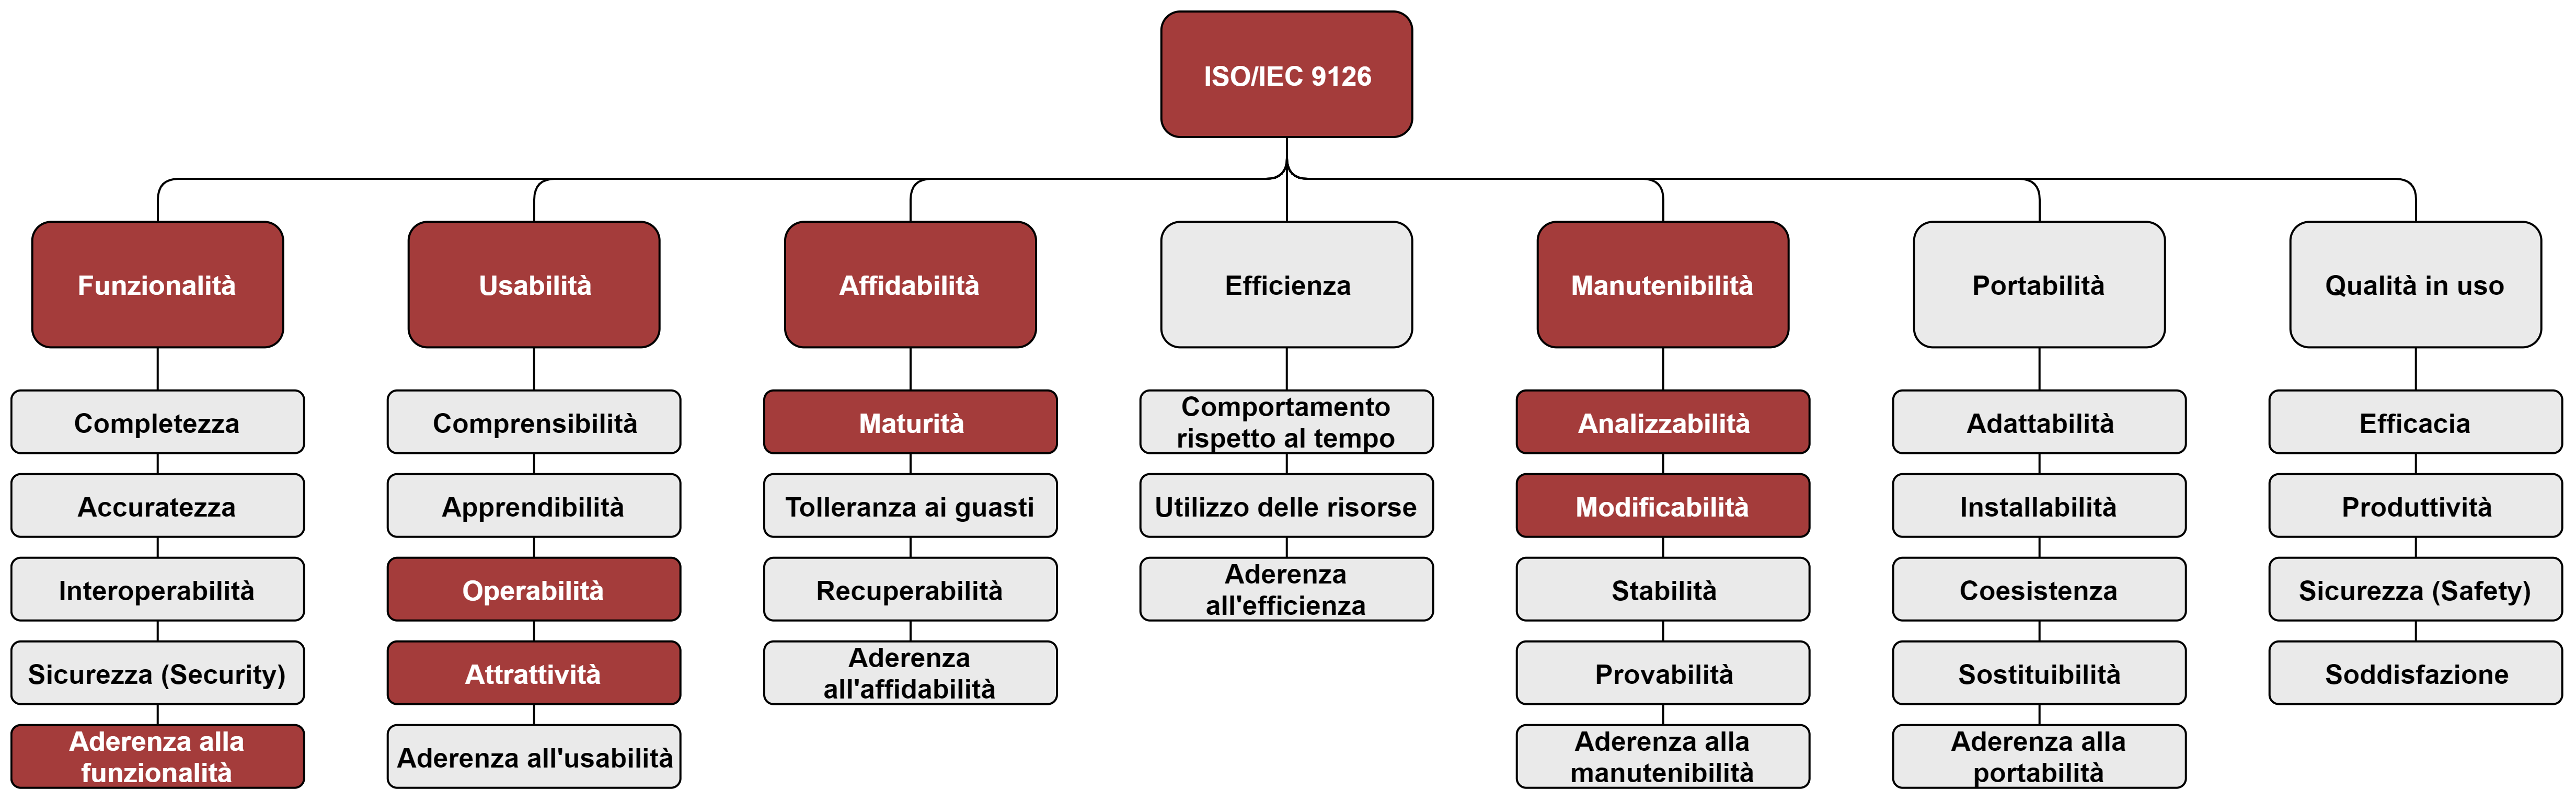
\includegraphics[scale=0.53]{Immagini/IsoIec9126.png}
    \caption{Schema dello standard ISO/IEC 9126. In rosso sono indicate le caratteristiche e attributi di interesse per il progetto.}
\end{figure}

\subsubsection{Metriche esterne}
Le metriche relative alla qualità "esterna" indirizzano le caratteristiche esteriori del software, cioè quelle rilevabili direttamente dagli utenti e dagli operatori.

\subsubsection{Metriche interne}
 Le metriche della qualità "interne" del software sono utilizzate durante la fase di sviluppo e permettono di valutare il comportamento del software dal punto di vista degli sviluppatori e di predire quello che sarà il punto di vista esterno degli utenti.

\subsubsection{Funzionalità}
Capacità del prodotto software di fornire funzioni adeguate al contesto di applicazione.
\begin{itemize}
\item \textbf{Adeguatezza}: Capacità di fornire un insieme di funzioni che permettano agli utenti del software di poter svolgere i loro compiti.
\item \textbf{Accuratezza}: Capacità di fornire i risultati attesi dall’utente con la precisione richiesta.
\item \textbf{Interoperabilità}: Capacità di interagire con uno o più sistemi specificati.
\item \textbf{Sicurezza (Security)}: Capacità di proteggere le informazioni e i dati dell’utente da persone non autorizzate ad accedervi.
\item \textbf{Aderenza alla funzionalità}: Capacità di aderire a standard, norme, convenzioni e regolamenti sulle funzionalità.
\end{itemize}

\subsubsection{Affidabilità}
Capacità del prodotto software di mantenere il livello di prestazione quando usato in condizioni specificate.
E’ limitata da errori nei requisiti, nella progettazione e nel codice del software.
\begin{itemize}
\item \textbf{Maturità}: Capacità di evitare che si verifichino errori.
\item \textbf{Tolleranza a guasti}: Capacità di mantenere il livello di prestazioni in caso di errori o violazione delle interfacce. Assieme alla \glo{Maturità}, descrivono l’attributo \glo{Disponibilità}, non specificato in quanto formato da questi due.
\item \textbf{Recuperabilità}: Capacità di ripristinare il livello di prestazioni e i dati in caso di errori e malfunzionamenti.
\item \textbf{Aderenza all’affidabilità}: Capacità di aderire a standard, norme, convenzioni e regolamenti sull’affidabilità.
\end{itemize}

\subsubsection{Usabilità}
Capacità del prodotto software di essere comprensibile, di poter essere studiato.
\begin{itemize}
\item \textbf{Comprensibilità}: Capacità di permettere all’utente di capire le funzionalità e come usarle con successo;
\item \textbf{Apprendibilità}: Capacità di permettere all’utente di imparare l’applicazione;
\item \textbf{Operabilità}: Capacità di permettere all’utente di usare il software e controllarlo;
\item \textbf{Attrattività}: Capacità di risultare attraente (ossia possedere una interfaccia utente accattivante);
\item \textbf{Aderenza all’usabilità}: Capacità di aderire a standard, norme, convenzioni e regolamenti sull’usabilità.
\end{itemize}

\subsubsection{Efficienza}
Capacità del prodotto software di realizzare le funzioni richieste nel minor tempo possibile.
\begin{itemize}
\item \textbf{Comportamento rispetto al tempo}: Capacità di fornire in tempi adeguati risposte per l’utente;
\item \textbf{Utilizzo risorse}: Capacità di utilizzare un appropriato numero e tipo di risorse, eseguendo le funzionalità previste;
\item \textbf{Aderenza all’efficienza}: Capacità di aderire a standard, norme, convenzioni e regolamenti sull’efficienza.
\end{itemize}

\subsubsection{Manutenibilità}
Capacità del prodotto software di essere modificato.
\begin{itemize}
\item \textbf{Analizzabilità}: Capacità di poter diagnosticare errori e individuare malfunzionamenti;
\item \textbf{Modificabilità}: Capacità di consentire lo sviluppo di modifiche al software originale;
\item \textbf{Stabilità}: Capacità di evitare effetti non desiderati;
\item \textbf{Provabilità}: Capacità di consentire la verifica delle funzionalità del prodotto software;
\item \textbf{Aderenza alla manutenibilità}: Vpacità di aderire a standard, norme, convenzioni e regolamenti sulla manutenibilità.
\end{itemize}

\subsubsection{Portabilità}
Capacità di essere trasportato da un ambiente ad un altro.
\begin{itemize}
\item \textbf{Adattabilità}: Verrà descritta se ce ne sarà il bisogno;
\item \textbf{Installabilità}: Verrà descritta se ce ne sarà il bisogno;
\item \textbf{Coesistenza}: Verrà descritta se ce ne sarà il bisogno;
\item \textbf{Aderenza alla portabilità}: Verrà descritta se ce ne sarà il bisogno.
\end{itemize}

\subsubsection{Qualità in uso}
\begin{itemize}
\item \textbf{Efficacia}: Capacità per l’utente del prodotto software di raggiungere obiettivi specifici con \glo{accuratezza} e \glo{completezza};
\item \textbf{Produttività}: Capacità di permettere all’utente di impegnare un numero definito di risorse, in relazione all’efficienza raggiunta. Queste risorse possono essere tempo, materiali e costi;
\item \textbf{Sicurezza fisica (Safety)}: Capacità di raggiungere un livello accettabile di rischio per dati, business e persone. I rischi sono tipicamente correlati a difetti in progettazione o analisi o codifica;
\item \textbf{Soddisfazione}: Capacità di soddisfare gli utenti in uno specifico contesto.
\end{itemize}
\subsubsection{Piano di Qualifica}
Nel documento \PdQ{} il gruppo \Gruppo{} illustra come intende gestire la qualità di processo e di qualità di prodotto, elenca le varie metriche definite per aderire alle definizioni degli standard e i test per verificare la corretta soddisfazione dei requisiti del prodotto software.\newline
La qualità di processo e la qualità di prodotto sono due aspetti chiaramente coordinati, ma vengono gestiti separatamente.
Le sezioni principali del documento sono le seguenti:
\begin{itemize}
    \item \textbf{Qualità di processo:} Sezione dove vengono elencate le metriche inerenti ai \glo{processi};
    \item \textbf{Qualità di prodotto:} Sezione dove vengono elencate le metriche inerenti al prodotto;
    \item \textbf{Strategia di testing:} Sezione dove viene elencato il piano di testing delle componenti e del sistema software nel suo complesso;
    \item \textbf{Standard di qualità adottati:} Sezione dove vengono spiegati gli standard adottati.
\end{itemize}
\paragraph{Garanzie sul prodotto}
\begin{itemize}
    \item Deve essere garantito che tutti i requisiti richiesti dal capitolato siano documentati, rispettino il contratto, siano coerenti ed eseguiti come richiesto dal proponente;
    \item Deve essere garantito che il prodotto software e la relativa documentazione siano conformi al capitolato e aderire ai requisiti.
    \item In preparazione alla consegna del prodotto software, deve essere garantito che esso soddisfatti i requisiti contrattuali.
\end{itemize}
\subsubsection{Metriche di qualità}
\paragraph{Codici metriche}\mbox{}
Ogni metrica di \glo{processo} ha un codice univoco ed è strutturato in questo formato:
\begin{center}
    M[Destinazione][Numero progressivo]
\end{center}
con:
\begin{itemize}  
    \item \textbf{[Destinazione]}:
    \begin{itemize}
        \item \textbf{PC}: Se la metrica fa riferimento al \glo{processo};
        \item \textbf{PD}: Se la metrica fa riferimento al prodotto.
    \end{itemize}
    \item \textbf{[Numero progressivo]}: Il numero della metrica in relazione alla sua destinazione, progressivo perché diverso per ogni metrica e in serie. Il conteggio parte da 1.
\end{itemize}

\paragraph{Struttura descrittiva metriche}
La seguente è una struttura ad elenco che descrive una metrica di processo o di prodotto. \\
I punti dell'elenco racchiusi fra parentesi quadre indicano che tale punto è opzionale e va inserito solo se necessario.\\
Inoltre, \textbf{Processo di riferimento} deve essere presente solo nelle metriche della qualità di processo, mentre \textbf{Attributo di riferimento} solo per la qualità di prodotto.
elencata in una lista, mentre il nome della metrica rappresenta il titolo di questo elenco ed è visibile nell'indice del documento. La struttura è la seguente:
\begin{itemize}
    \item \textbf{Codice}: Codice univoco;
    \item \textbf{Descrizione}: Breve descrizione della metrica e del contesto applicativo;
    \item \textbf{Processo di riferimento}: Viene indicata in quale \glo{processo} viene applicata tale metrica (riferendosi allo standard);
    \item \textbf{Attributo di riferimento}: Viene indicato in quale attributo della caratteristica di prodotto viene applicata tale metrica (riferendosi allo standard);
    \item \textbf{Sigla}: nome della metrica sotto forma di acronimo, utilizzato principalmente nelle formule matematiche e nei range di accettazione;
    \item \textbf{[Formula:} formula matematica per poter calcolare il valore della metrica];
    \item \textbf{Range di valori che può assumere}: sezione in cui sono descritti i range di accettazione per i valori delle metriche.
    \begin{itemize}
        \item \textbf{Accettabile}: range in cui i valori della metrica possono essere ritenuti accettabili per garantire la qualità;
        \item \textbf{Ottimale}: range in cui i valori della metrica possono essere ritenuti ottimali per garantire la qualità.
    \end{itemize}
\end{itemize}

\paragraph{Metriche di processo}
Per monitorare l'aderenza ai processi dallo standard ISO/IEC 12207 istanziati, vengono utilizzate delle metriche. Il Responsabile, grazie ai valori ricavati dalle metriche, è facilitato nel valutare il \glo{processo} e di effettuare, se necessario, modifiche alla pianificazione.

\paragraph{Metriche di prodotto}
Il modello di qualità del software descritto dallo standard ISO/IEC 9126 definisce le caratteristiche e gli attributi del prodotto software, ciascuna misurabile da metriche interne (che richiedono la disponibilità del codice sorgente - white box) o esterne (che richiedono il prodotto software in esecuzione - black box).
Una volta specificati i requisiti di qualità del prodotto software, si identificano le caratteristiche e attributi di qualità che più contribuiscono a verificare l'aderenza allo standard e ai requisiti.
Il gruppo \Gruppo{} si è impegnato a scegliere le metriche interne che maggiormente influenzano (in positivo) le caratteristiche esterne del prodotto finale, in modo che esse possano predire quanto più possibile la qualità del risultato finale. 

\paragraph{Tabella riassuntiva metriche}
Per riassumere tutte le metriche e le loro caratteristiche descritte all'interno del \PdQ{}, alla fine della sezione in cui vengono illustrate vi sono delle tabelle riassuntive che hanno questa struttura:
{
\rowcolors{2}{grigetto}{white}
\renewcommand{\arraystretch}{1.5}
\begin{longtable}{ c C{4cm} c C{3.5cm} C{3.5cm}}
\caption{Tabella metriche dei processi/prodotti}\\
\rowcolor{darkblue}
\textcolor{white}{\textbf{Metrica}} & \textcolor{white}{\textbf{Nome}} & \textcolor{white}{\textbf{Sigla}} & \textcolor{white}{\textbf{Range Accettabile}} & \textcolor{white}{\textbf{Range Ottimale}}\\
Codice & Nome della metrica & Sigla & Range Accettabile & Range Ottimale \\
\end{longtable}
}

\subsubsection{Lista delle metriche di processo}
\paragraph{Processi di supporto}

\subparagraph{Verifica}
\subsubparagraph{Metrica - Code coverage}
\begin{itemize}
	\item \textbf{Codice:} MPC7
	\item \textbf{Descrizione:} È la percentuale di copertura del codice attraversato dai test rispetto al totale del codice di base. Per dare una misurazione in termini di grandezza si adoperano le linee di codice come riferimento;
	\item \textbf{Processo di riferimento:} \glo{Processi} di verifica;
	\item \textbf{Sigla:} $CC$
	\item \textbf{Formula:} $$CC = \frac{|linee \; di \; codice \; percorse \; dai  \; test|}{|linee \; di \; codice \; totali|} \; \cdot \; 100$$
	\item \textbf{Strumenti utilizzati:} \glo{SonarQube}.
\end{itemize}
   \paragraph{Processi organizzativi}

\subparagraph{Pianificazione}

\subsubparagraph{Metrica - Actual Cost of Work Performed}
    \begin{itemize}
        \item \textbf{Codice:} MPC8
        \item \textbf{Descrizione:} Denaro speso fino al momento del calcolo;
        \item \textbf{Processo di riferimento:} Gestione;
        \item \textbf{Sigla:} $ACWP$
        \item \textbf{Formula:} $$ACWP = {Sommatoria\; delle\; ore\; lavorative\; moltiplicate\; con\; il\; corrispondente\; costo\; orario}$$
        \item \textbf{Strumenti utilizzati:} Fogli Google.
    \end{itemize}

\subsubparagraph{Metrica - Budgeted Cost of Work Scheduled}
\begin{itemize}
	\item \textbf{Codice:} MPC9
    \item \textbf{Descrizione:} Costo pianificato per realizzare le attività di progetto pianificate fino al momento del calcolo.
    Per attività di progetto pianificate si intendono il numero di requisiti che devono soddisfatti dal prodotto software;
	\item \textbf{Processo di riferimento:} Gestione;
	\item \textbf{Sigla:} $BCWS$
	\item \textbf{Formula:} $$BCWS = {B_{tot} * \% \;di\; lavoro\; pianificato}$$
	con:
	\begin{itemize}
		\item $B_{tot}$ = Budget totale.
	\end{itemize}
	\item \textbf{Strumenti utilizzati:} Fogli Google.
\end{itemize}

\subsubparagraph{Metrica - Budgeted Cost of Work Performed}
\begin{itemize}
	\item \textbf{Codice:} MPC10
	\item \textbf{Descrizione:} Il costo del lavoro fatto fino al momento del calcolo, ovvero la variazione del numero di requisiti soddisfatti nel periodo in cui la metrica viene calcolata;
	\item \textbf{Processo di riferimento:} Gestione;
	\item \textbf{Sigla:} $BCWP$
	\item \textbf{Formula:} $$BCWP = {B_{tot} * \% \;di\; lavoro\; svolto}$$
	con:
	\begin{itemize}
		\item $B_{tot}$ = Budget totale.
	\end{itemize}
	\item \textbf{Strumenti utilizzati:} Fogli Google.
\end{itemize}

    \subsubparagraph{Metrica - Schedule variance}
    \begin{itemize}
        \item \textbf{Codice:} MPC11
        \item \textbf{Descrizione:} È il valore che indica se si è in linea ($=0$), in anticipo ($>0$) oppure in ritardo ($<0$) rispetto alla schedulazione delle attività di progetto pianificate nella \glo{baseline};
        \item \textbf{Processo di riferimento:} Gestione;
        \item \textbf{Sigla:} $SV$
        \item \textbf{Formula:} $$SV = {BCWP \; - \; BCWS}$$
        con:
        \begin{itemize}
            \item $BCWP$ = Budgeted Cost of Work Performed (valore delle attività eseguite nella data corrente);
            \item $BCWS$ = Budgeted Cost of Work Scheduled (costo pianificato per la realizzazione delle attività di progetto alla data corrente);
        \end{itemize}
    \item \textbf{Strumenti utilizzati:} Fogli Google.
    \end{itemize}

    \subsubparagraph{Metrica - Budget variance}
        \begin{itemize}
            \item \textbf{Codice:} MPC12
            \item \textbf{Descrizione:} È il valore che indica se alla data corrente si è speso di più ($>0$) o di meno ($<0$) rispetto a quanto pianificato dal budget totale $B_{tot}$;
            \item \textbf{Processo di riferimento:} Gestione;
            \item \textbf{Sigla:} $BV$
            \item \textbf{Formula:} $$BV = {BCWS \; - \; ACWP}$$
            con:
            \begin{itemize}
                \item $BCWS$ = Budgeted Cost of Work Scheduled (costo pianificato per la realizzazione delle attività di progetto alla data corrente);
                \item $ACWP$ = Actual Cost of Work Performed (costo effettivamente sostenuto alla data corrente);
                \item $B_{tot}$ = Budget totale.
            \end{itemize}
        \item \textbf{Strumenti utilizzati:} Fogli Google.
        \end{itemize}
\newpage
\subsubsection{Lista delle metriche di prodotto}
\paragraph{Metriche interne}
Le metriche della qualità "interne" del software sono utilizzate durante la fase di sviluppo e permettono di valutare il comportamento del software dal punto di vista degli sviluppatori e di predire quello che sarà il punto di vista esterno degli utenti.

\subparagraph{Usabilità}
Capacità del prodotto software di essere comprensibile, di poter essere usato e compreso facilmente, in ogni sua parte, da qualsiasi utente che lo voglia usare.\\

\subsubparagraph{Metrica - Attrattività della User Interface (UI)} 
\begin{itemize}
    \item \textbf{Codice:} MPD1
    \item \textbf{Descrizione:} Misurare quanto attrattive risultino le interfacce agli utenti dal punto di vista grafico.
    Gli utenti dovranno poi compilare un questionario in base all'esperienza che hanno fatto;
    Il valore medio di tale valutazione è ritenuto valido se almeno tre utenti hanno compilato il questionario. 
    Viene utilizzata una scala a quattro valori: Molto attrattivo, Attrattivo, Poco attrattivo, Non Attrattivo;
    \item \textbf{Attributo di riferimento:} \glo{Attrattività};
    \item \textbf{Sigla:} $AUI$
    \item \textbf{Formula:}$$AUI = V(q) $$
    con:
        \begin{itemize}
        \item $V$ = Valore medio dei risultati;
        \item $q$ = Questionario compilato;
        \end{itemize}
    \item \textbf{Strumenti utilizzati:} Moduli Google.
\end{itemize}

\subparagraph{Manutenibilità}
Capacità di predire il livello di impegno richiesto per modificare il prodotto software dal punto di vista degli sviluppatori.           
\subsubparagraph{Metrica - Complessità Ciclomatica del Software} 
    \begin{itemize}
    \item \textbf{Codice:} MPD2
    \item \textbf{Descrizione:} Misurare la complessità ciclomatica dei singoli moduli sviluppati;
    \item \textbf{Attributo di riferimento:} \glo{Modificabilità};
    \item \textbf{Sigla:} $CCS$
    \item \textbf{Formula:} $$CCS = e - n + p$$
    con:
    \begin{itemize}
        \item $G$ = grafo del modulo;
        \item $e$ = numero di congiunzioni tra statement (corrispondenti agli archi di un grafo);
        \item $n$ = numero di statement (nodi presenti nel grafo);
        \item $p$ = numero delle componenti connesse da ogni nodo (per esecuzione sequenziale: p=2, essendovi un predecessore e un successore);
    \end{itemize}
    \item \textbf{Strumenti utilizzati:} Non ancora definito.
\end{itemize}

\subsubparagraph{Metrica - Unità Documentate} 
\begin{itemize}
    \item \textbf{Codice:} MPD3
    \item \textbf{Descrizione:} Misurare in percentuale il numero di unità di codice con documentazione tecnica;
    \item \textbf{Attributo di riferimento:} \glo{Modificabilità};
    \item \textbf{Sigla:} $UD$
    \item \textbf{Formula:} $$UD = \frac{|unit\grave{a} \; di \; codice \; con \; documentazione \; tecnica|}{|unit\grave{a} \; di \; codice|} \cdot 100$$
    \item \textbf{Strumenti utilizzati:} Non ancora definito.
\end{itemize}
              
       
\paragraph{Metriche esterne}
Le metriche relative alla qualità "esterna" indirizzano le caratteristiche esteriori del software, cioè quelle rilevabili direttamente dagli utenti e dagli operatori.

\subparagraph{Affidabilità}
Capacità del prodotto software di dimostrare un adeguato livello di affidabilità quando opererà nel sistema in cui è previsto debba operare.
  
\subsubparagraph{Metrica - Presenza di code smell} 
\begin{itemize}
    \item \textbf{Codice:} MPD4
    \item \textbf{Descrizione:} Misurare il numero di \glo{code smell} presenti all'interno del codice del prodotto;
    \item \textbf{Attributo di riferimento:} \glo{Manutenibilità};
    \item \textbf{Sigla:} $CS$
    \item \textbf{Formula:} $$CS = {numero \; di \; code \; smell \; rilevati}$$
    \item \textbf{Strumenti utilizzati:} \glo{SonarQube}.
\end{itemize}

\subsubparagraph{Metrica - Presenza di vulnerabilità} 
\begin{itemize}
    \item \textbf{Codice:} MPD5
    \item \textbf{Descrizione:} Misurare il numero di \glo{vulnerabilità} presenti all'interno del codice del prodotto;
    \item \textbf{Attributo di riferimento:} \glo{Sicurezza};
    \item \textbf{Sigla:} $VLN$
    \item \textbf{Formula:} $$VLN = {numero \; di \; vulnerabilit\grave{a} \; rilevate}$$
    \item \textbf{Strumenti utilizzati:} \glo{SonarQube}.
\end{itemize}

\subsubparagraph{Metrica - Presenza di bug} 
\begin{itemize}
    \item \textbf{Codice:} MPD6
    \item \textbf{Descrizione:} Misurare il numero di \glo{bug} presenti all'interno del codice del prodotto;
    \item \textbf{Attributo di riferimento:} \glo{Operabilità};
    \item \textbf{Sigla:} $BUG$
    \item \textbf{Formula:} $$BUG = {numero \; di \; bug \; rilevati}$$
    \item \textbf{Strumenti utilizzati:} \glo{SonarQube}.
\end{itemize}

\subsubparagraph{Metrica - Maturità dei Test} 
\begin{itemize}
    \item \textbf{Codice:} MPD7
    \item \textbf{Descrizione:} Misurare la percentuale di casi di test eseguiti con successo rispetto al numero totale previsto per garantire piena copertura dei requisiti sia funzionali che qualitativi(usabilità, affidabilità, efficienza);
    \item \textbf{Attributo di riferimento:} \glo{Maturità};
    \item \textbf{Sigla:} $MT$
    \item \textbf{Formula:} $$MT = \frac{|casi \; di \; test \; eseguiti \; con \; successo|}{|casi \; di \; test \; previsti|} \cdot 100$$
    \item \textbf{Strumenti utilizzati:} Non ancora definito.
\end{itemize}
       
\subparagraph{Usabilità}
Capacità del prodotto software di essere facilmente comprensibile, apprendibile ed operabile per ogni utente intenzionato a usarlo.

\subsubparagraph{Metrica - Profondità Strutturale dell'Interfaccia}
\begin{itemize}
    \item \textbf{Codice:} MPD8
    \item \textbf{Descrizione:} È sconsigliato per le interfacce utente l'utilizzo di una struttura troppo profonda per questioni di usabilità. L'utente non deve fare troppi passaggi per raggiungere la funzionalità desiderata;
    \item \textbf{Attributo di riferimento:} \glo{Operabilità};
    \item \textbf{Sigla:} $PSI$
    \item \textbf{Strumenti utilizzati:} Controllo manuale.
\end{itemize}